\documentclass[conference]{IEEEtran}
\IEEEoverridecommandlockouts
% The preceding line is only needed to identify funding in the first footnote. If that is unneeded, please comment it out.
\usepackage{cite}
\usepackage{amsmath,amssymb,amsfonts}
\usepackage{algorithmic}
\usepackage{graphicx}
\usepackage{textcomp}
\usepackage{xcolor}
\def\BibTeX{{\rm B\kern-.05em{\sc i\kern-.025em b}\kern-.08em
    T\kern-.1667em\lower.7ex\hbox{E}\kern-.125emX}}

\usepackage{graphicx}
\usepackage{float}
\usepackage{multirow}  %% For table
\usepackage{amsmath}
\usepackage{float}
\usepackage{mathtools}
\usepackage{subfig}
\usepackage{algorithm}
\usepackage[noend]{algpseudocode}
\usepackage{breqn}
\usepackage{hyperref}
\usepackage{amssymb}
\usepackage[export]{adjustbox}
\def\algbackskip{\hskip-\ALG@thistlm}
\DeclareMathOperator*{\argmin}{arg\,min}
\newcommand{\norm}[1]{\left\lVert#1\right\rVert}
\usepackage[switch]{lineno}
\renewcommand{\linenumberfont}{\normalfont\bfseries\small\color{blue}}
\linenumbers
\setcounter{page}{1} 
\begin{document}
%
\title{Towards Searching Efficient Architecture Sizes for Neural Networks in Binary Classification Problems}

\author{\IEEEauthorblockN{1\textsuperscript{st} Given Name Surname}
\IEEEauthorblockA{\textit{dept. name of organization (of Aff.)} \\
\textit{name of organization (of Aff.)}\\
City, Country \\
email address or ORCID}
\and
\IEEEauthorblockN{2\textsuperscript{nd} Given Name Surname}
\IEEEauthorblockA{\textit{dept. name of organization (of Aff.)} \\
\textit{name of organization (of Aff.)}\\
City, Country \\
email address or ORCID}
\and
\IEEEauthorblockN{3\textsuperscript{rd} Given Name Surname}
\IEEEauthorblockA{\textit{dept. name of organization (of Aff.)} \\
\textit{name of organization (of Aff.)}\\
City, Country \\
email address or ORCID}
\and
\IEEEauthorblockN{4\textsuperscript{th} Given Name Surname}
\IEEEauthorblockA{\textit{dept. name of organization (of Aff.)} \\
\textit{name of organization (of Aff.)}\\
City, Country \\
email address or ORCID}
\and
\IEEEauthorblockN{5\textsuperscript{th} Given Name Surname}
\IEEEauthorblockA{\textit{dept. name of organization (of Aff.)} \\
\textit{name of organization (of Aff.)}\\
City, Country \\
email address or ORCID}
\and
\IEEEauthorblockN{6\textsuperscript{th} Given Name Surname}
\IEEEauthorblockA{\textit{dept. name of organization (of Aff.)} \\
\textit{name of organization (of Aff.)}\\
City, Country \\
email address or ORCID}
}

\maketitle
\thispagestyle{plain}
\pagestyle{plain}
\begin{abstract}

In recent years, deep neural networks have had great success in machine learning and pattern recognition. Architecture size for a neural network has long been treated as complete hyper-parameter with little study about it and yet this parameter contributes significantly to the success of any neural network. In this study, we optimize this hyper-parameter by studying different search algorithms to find a neural network architecture size that would give the highest accuracy. We specifically apply linear search and binary search on two well-known binary classification problems and compare the results. We also propose how to relax some of the assumptions regarding the dataset for these binary classification problems so that our solution can be generalized to any binary classification problem. By finding the optimal architecture size for any binary classification problem fast, we hope that our research creates a framework to optimize a model for any binary classification problem.

\begin{IEEEkeywords}
Binary Search, Architecture Size, Maximizing Accuracy, Binary Classification Problems
\end{IEEEkeywords}
\end{abstract}


\section{Introduction}
In recent decades, advances in deep neural networks (DNNs) have allowed computers to achieve or even exceed human-level performance on difficult image recognition tasks. 
Breakthrough in many challenging applications, such as speech recognition (Hinton et al., 2012), image recognition (LeCun et al., 1998;
Krizhevsky et al., 2012) and machine translation (Sutskever et al., 2014; Bahdanau et al., 2015; Wu
et al., 2016) have been achieved due to designing architectures that are efficient for the task at hand as [https://arxiv.org/pdf/1611.01578.pdf] states.

One such shift is for example in computer vision to predict objects in images by AlexNet (Krizhevsky
et al., 2012), VGGNet (Simonyan \& Zisserman, 2014), GoogleNet (Szegedy et al., 2015), and
ResNet (He et al., 2016a) which replaced the previously used architecture designs that were based on features such as SIFT (Lowe, 1999), and HOG (Dalal \& Triggs, 2005). Although designing architectures for a specific problem and dataset enabled greater success, models and architectures got more complicated and started to require many hyper-parameters, which are parameters that user decides. These hyper-parameters such as number of hidden layers, number of nodes at each layer etc affects the accuracy, model training duration and architecture size directly, yet focus given to these hyper-parameters have been little. In this study, we search for architecture sizes that would give the highest accuracy and lowest training time for a given dataset. 

Our aim is to look at the architecture size as a hyper-parameter and propose a framework of understanding to come up with a model architecture for a given problem. We specifically consider the number of hidden layers and the number of neurons at each layer for a given problem and we search to locate the the optimal number of units and number of layers in a deep neural network (DNN). We use binary search and linear search as a way of finding the optimal architecture size and study binary classification problems so that the output layer for all the datasets we look has only one neuron. We use Titanic dataset and a Customer Churn dataset to compare our findings. 

This paper is organized such that Section \ref{relatedwork} discusses related work, Section \autoref{methodology} discusses datasets and search algorithms used, Section \autoref{experimentandresults} reports the experiments and results and finally Section \autoref{conclusion} concludes the paper by going over the important findings one more time.


\section{Related Work} \label{relatedwork}

Architecture size has long been considered a hyper-parameter that user picks randomly. Yet, this hyper-parameter impacts the model accuracy for a given problem significantly. Recent years have shown several studies hyper-parameters are optimized ((Bergstra et al., 2011; Bergstra \& Bengio, 2012; Snoek et al., 2012; 2015; Saxena \&
Verbeek, 2016). Such studies have been limited to fixed-size models when searching for the optimal hyper-parameters. 

[https://arxiv.org/abs/1611.01578] relaxed that fixed-space assumption searching for the optimal architecture size via reinforcement learning. [https://arxiv.org/pdf/1909.07378.pdf] has studied binary neural networks to only look at the neural networks that are compact. These studies have proposed new frameworks in determining the architecture size for neural networks in a systematic way rather than leaving such choice as completely hyper-parameter. However, current studies have taken different assumptions regarding the models they design when applying their approach. Wheng et al. added a constraint for the type of neural networks that they are studying so that they only studied binary neural networks when determining the optimal architecture size to give the highest accuracy. Binary neural networks are neural networks where the weights consist of only +1 and -1 values.
The constraint that they added is close to what we added. However, we don't force binarization on the weights, we only force such binarization on the output layer since we are only tackling binary classification problems in this study.

 
\section{Methodology} \label{methodology}

Because of the fact that convolutional neural networks (CNN) require training and testing on typically a large data set, it becomes increasingly difficult and time consuming to determine optimal hyper-parameters. Although there are methods to search this hyper-parameter (search) space, none have successfully implemented a binary search method. 

In this work, we define model evaluation as the end-to-end training and testing of a model architecture with a constant training and testing data set, which is specially outlined in Figure \autoref{datasetaummption}. 



\subsection{Assumptions}
\subsubsection{Network Architecture Assumption}
We will be modeling our classification problem with an input layer, one hidden layer, and one output layer as shown below.
Add figure later.
\begin{figure}[H]
    \centering
    \includegraphics{figures/placeholder.png}
    \caption{Caption}
    \label{fig:my_label}
\end{figure}

\subsubsection{Accuracy Distribution Assumption}

Our first general assumption is that the accuracy maximum is uni-modal with respect to the number of units, $n$, in the hidden layer. This implies that there exists one maximum between $1$ and $n$. Furthermore, we assume that this distribution exists as a cusp  distribution where the slope of the distribution is monotonically increasing in magnitude as the maximum accuracy is approached form either side of the distribution.

\subsubsection{Data Set Assumptions} \label{datasetaummption}

With respect to our data set, we assume that there will be $m$ number of inputs but only $1$ output unit in the output layer. As a result, we are simplifying this to only binary classification problems. We suspect that specifically our linear search method in Figure \autoref{linearsearch} will be more efficient for smaller input spaces, whereas our binary search method in Figure \autoref{binarysearch} will be more efficient for larger input spaces. It follows that we can explore the relative speeds of these two methods under our respective assumptions in order to determine a general threshold for when method should be used over the other.

\subsection{Churn Dataset}
Churn dataset is a dataset made public by Drexel Society of Artificial Intelligence\cite{churndataset}. It has 14 columns and 10000 rows where each row has information for a business that uses a cloud service and each column represents one feature regarding the customer. The dataset has specifically 14 columns but 3 of them are row number, customer id and company name which are excluded during the training process because they don't have meaning for the model. Out of remaining columns are features to indicate the revenue of the customer, contract duration of the customer, whether the customer has raised a ticket or renewed the contract before etc. The model that is trained on this dataset predicts whether the customer will leave the service contract or not. So, the label column is either 0 or 1 to indicate if the customer will renew the service. We train a model that has 1 input layer that consist of 11 nodes, one hidden that consists of D nodes and 1 output layer that consist of 1 node. The methods we follow is to find the D that would give the maximum accuracy in our model first via linear search and second via (modified) binary search. 


\subsection{Titanic Dataset}
Titanic dataset is a dataset made public by Kaggle \cite{titanickaggledataset}. It has 14 columns and 1310 rows where each row has information for a passenger on Titanic and each column is one of many features. The dataset has specifically 13 features such as sex, fare amount, ticket class, cabin type etc and the label for each sample that the model predicts is either 0 or 1 to indicate if the person survived or not. We train a model that has 1 input layer that consist of 13 nodes, one hidden that consists of D nodes and 1 output layer that consist of 1 node. The methods we follow is to find the D that would give the maximum accuracy in our model first via linear search and second via (modified) binary search. 

\begin{figure}[H]
    \centering
    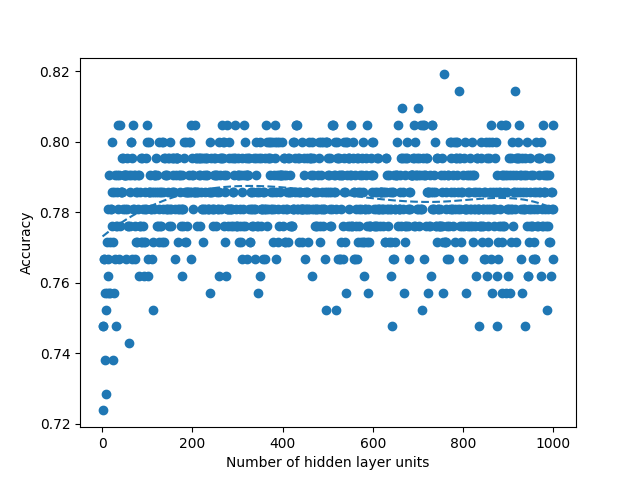
\includegraphics[width=0.8\linewidth]{figures/val_accuracy_titanic.png}
    \caption{Titanic Accuracy plot}
    \label{fig:titanic_accuracy}
\end{figure}


\subsection{Linear Search} \label{linearsearch}
For each model, we have a varying hidden layer of dimension D between the input layer and the output layer. We sweep D from 1 to 1000 to find the maximum accuracy which we treat as our baseline. Such linear search takes exactly 1000 steps meaning we need to train and test 1000 models with different architectures to find the highest accuracy for this binary classification problem. We then assume the accuracies are indeed partially sorted and apply binary search to skip some number of model architectures which then helps us the training time reduce by 90 times and achieves a maximum accuracy in around 11 steps. We discuss ways of applying binary search to this problem in section \ref{binarysearch}.

Usage of linear search is considered baseline in our study for two datasets that we investigated. Linear search is considered baseline/brute force way because when we apply linear search to this problem of finding an accurate representation, we are iterating over all the elements in the array and checking if the current element is greater than the maximum element that we have seen so far. We pick a range to constrain the search space so that finding the number of hidden layer units is not a unbounded problem but a bounded problem. In this study, we picked the range to go from 0 to 1000 because two datasets that we studied had 14 and 11 dimensions in their input layer, and the output layer had 1 dimension because both datasets were modeled to solve a binary classification problem. Therefore, the output layer was 0 or 1. In our studies, 1000 proved to be effective as the upper layer because we haven't realized any benefits of going more than three orders of magnitude larger than the input dimensions in our problems. The time complexity for finding the maximum by iterating all over the elements to find the maximum is O(n) and colloquially, such linear search to find the maximum element took 1000 steps to find.  

\begin{algorithm}[H]
\caption{Finding maximum accurate architecture size in a neural network via linear search}
\begin{algorithmic}[1]
\Procedure{maximize_accuracy_linearly}{}
\STATE $\textit{n} \gets \text{upper bound of dimension in a hidden layer}$
\STATE $\textit{max\_accuracy} \gets 0$
\STATE $\textit{max\_network\_size} \gets 1$
\FOR{$current\_size$ := 1 to $max\_network\_size$} 
\STATE $\textit{current\_accuracy} \gets \textit{Pipeline(model(current\_size))}$
\IF {$\textit{current\_accuracy} \textit{>} \textit{max\_accuracy}$}
\STATE $max\_accuracy \gets current\_accuracy$
\STATE $max\_network\_size \gets current\_size$
\ENDIF
\ENDFOR
\RETURN $(max\_accuracy, max\_network\_size)$
\end{algorithmic}
\end{algorithm}



\subsection{Binary Search} \label{binarysearch}

Given our assumptions, the premise of the binary search method is to implement a way to determine from which side we are approaching the cusp. Because of the fact that the slope of the distribution is monotonically increasing in magnitude in approaching the maximum accuracy, we model the where each index of the search is based on the sign of the recorded slope and the previously recorded slopes in the search. 

In a normal binary search, one would use the $>$ and $<$ operators in order to remove parts of the search space. We perform this search in a similar way using slopes. Therefore, each comparison will take at least two model evaluations for each comparison. We introduce a dynamic variable $\delta$ that models the distance between each model evaluation taken at $n_i$ and $n_j$, which represent the current number of units on which we base our comparison and search. Figure \autoref{fig:binarysearch} models the relationship between these three variables in the search algorithm.

We then define  $\gamma_L$ and $\gamma_U$ which represent the minimum and maximum number of units in our search space, respectively. These variables will be used to keep track of the lower and upper bounds of our search. As shown in Figure \autoref{fig:binarysearch0}, these two variables are set to $1$ and $n$ by default. If the search continues appropriately, these will approach the cusp from either side.

Moreover, we define lists $m_L$ and $m_U$ for the previously recorded slopes for the lower and upper bound side of the maximum cusp, respectively. Initially, they are empty as displayed in Figure \autoref{fig:binarysearch0}. As the search advances, the previously recorded slopes will be appended to either list depending on which from side the slope was taken.

After initializing the variables, the search begins by performing two model evaluations at $n_i$ and $n_j$ in Figure \autoref{fig:binarysearch0}. This would result in a negative slope, which indicates that the upper bound conditions are changed as shown in Figure \autoref{fig:binarysearch1}. In this figure, the upper bound $\gamma_U$ is set to the $n$ from which the slope was estimated and the slope is appended to the list containing previously recorded slopes on the right side of the cusp, $m_U$. As displayed in this figure, the search continues to the opposite side of the search space.

\begin{figure}[H]
     \centering
     \subfloat[Binary hyperparameter search. Initial conditions.]{\label{fig:binarysearch0}{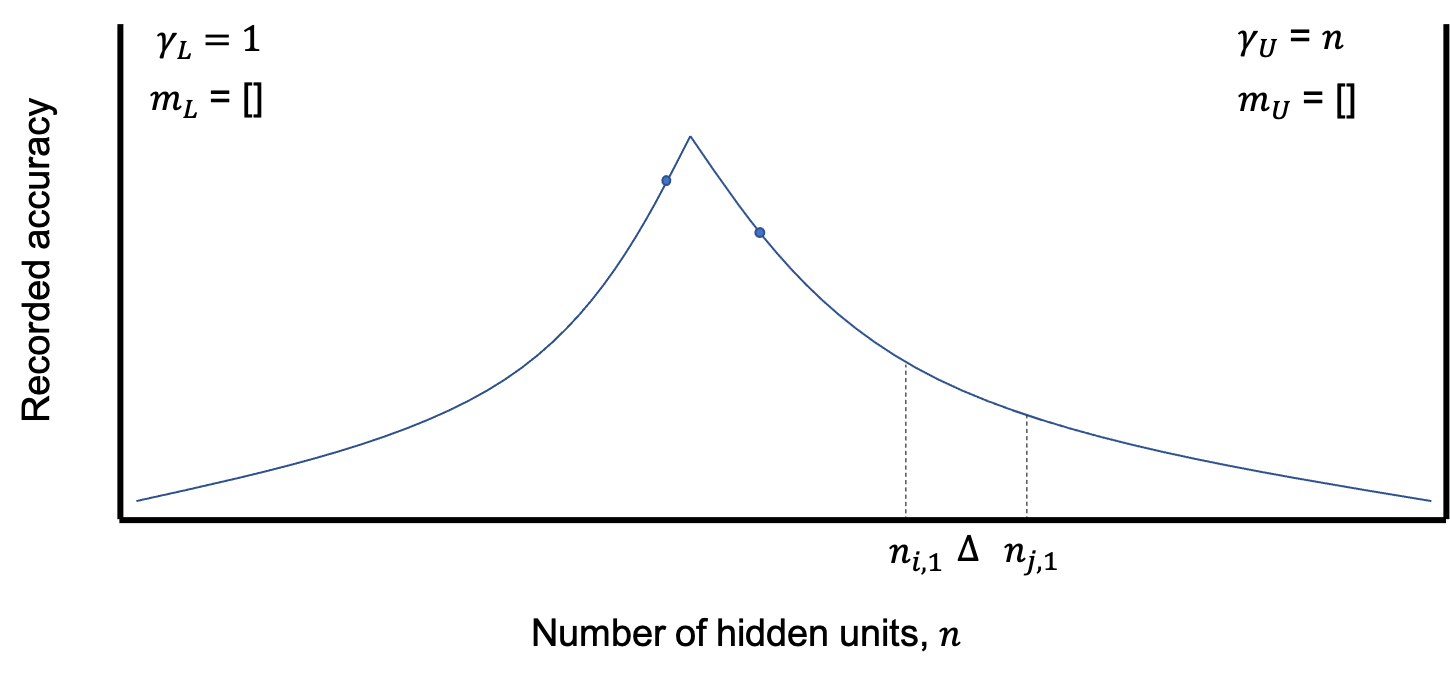
\includegraphics[width=0.8\linewidth]{figures/binarysearch0.png}}}\hfill
    \subfloat[Binary hyperparameter search. First comparison.]{\label{fig:binarysearch1}{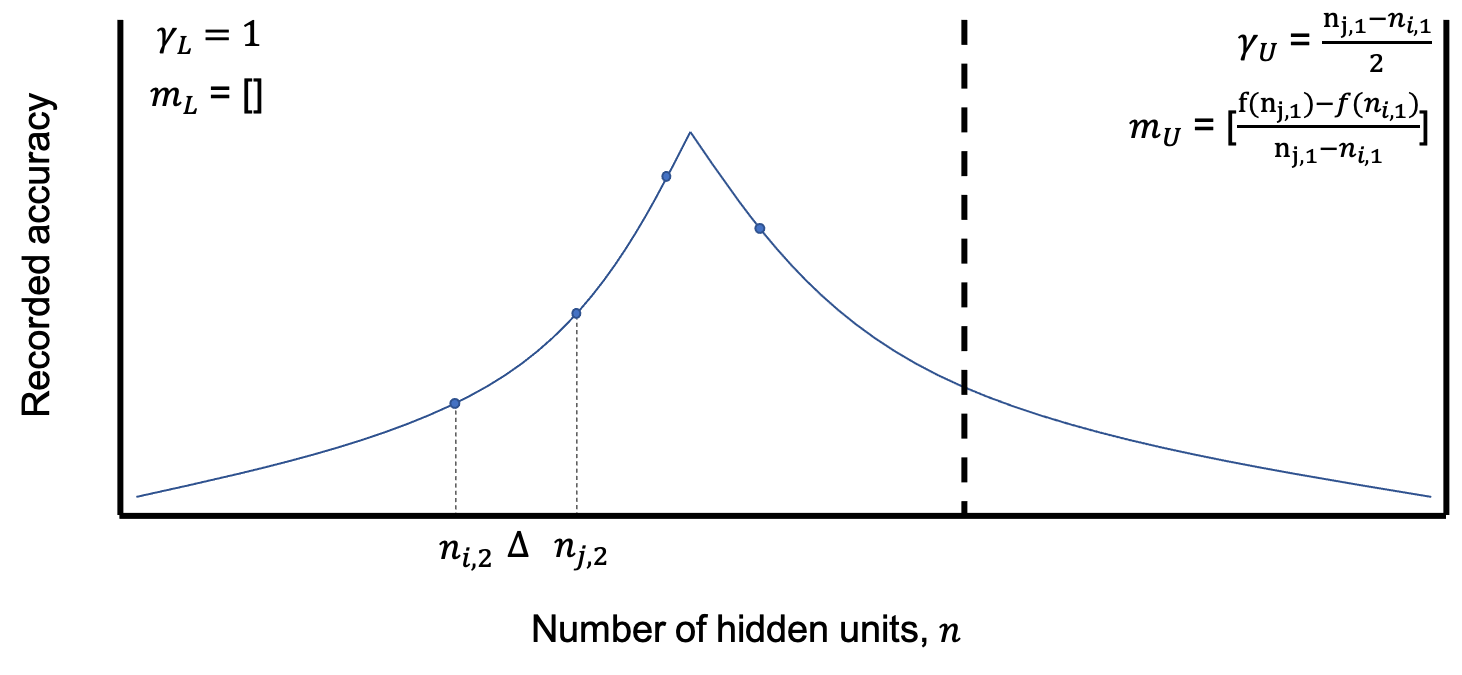
\includegraphics[width=0.8\linewidth]{figures/binarysearch1.png}}}
    \caption{Binary hyperparameter search.}
    \label{fig:binarysearch}
\end{figure}

After each slope is calculated, we want to know whether there is enough evidence to suggest that there exists a maximum either at or near that recorded slope. We determine the probability of a maximum by evaluating a posterior shown in \autoref{posteriorequ}. This probability can be broken down into a likelihood in \autoref{likelihoodequ} and a prior in \autoref{priorequ}.



4. Evaluate the following posterior for the probability of encountering the maximum accuracy in this distribution. 

5. Determine if there is sufficient evidence for a maximum within $n_i$ and $n_j$ by evaluating

Posterior:
\begin{equation}\label{posteriorequ}
\centering
\begin{aligned}
    P(maximum \mid m, \gamma_{L}, \gamma_{U}, \delta) = P(y{=}m {\mid} maximum) * \\
    p(maximum {\mid} \gamma_{L}, \gamma_{U}, \delta)
\end{aligned}
\end{equation}

Likelihood:
\begin{equation}\label{likelihoodequ}
    P(y=m \mid maximum) = N(\hat{y} = \beta_{0} + \beta_{1} * x, \sigma) 
\end{equation}

Prior:
\begin{equation}\label{priorequ}
    P(maximum \mid \gamma_{L}, \gamma_{U}, \delta) = \frac{\delta}{\gamma_{U} - \gamma_{L}}
\end{equation}

\begin{figure}[H]
    \centering
    \includegraphics[width=0.8\linewidth]{figures/binary_search_figure_1.png}
    \setlength{\belowcaptionskip}{-15pt}
    \caption{Binary search method. Temporary figure.}
    \label{dnadigest}
\end{figure}

Here are the general steps for the search we performed:
1. Run model 1 to $n$ to determine sufficient $\delta$ between $n_i$ and $n_j$ empirical. 

2. Track $\gamma_L$ and $\gamma_U$ through binary search (starting with $\frac{\gamma_{U} - \gamma_{L}}{2}$) and pick $n_i$ and $n_j$ so that $\frac{\gamma_{U} - \gamma_{L}}{2}$ is a midpoint between them.

3. In evaluating the slope resulting from $n_i$ and $n_j$, keep a list of $m_L$ and $m_U$ for the previously recorded slopes for the lower and upper bound, respectively.

\begin{algorithm}[H]
\caption{Measuring Jaccard Index with stride $\alpha$}\label{cnnscorestride}
\begin{algorithmic}[1]
\Procedure{$s_{\alpha}$}{}
\STATE $\textit{n} \gets \text{number of highest-scoring k-mers to analyze}$
\STATE $\textit{score} \gets 0$
\STATE $\textit{act\_outputs} \gets \text{actual outputs}$
\STATE $\textit{pred\_outputs} \gets \text{outputs from CNN}$
\STATE $\textit{act\_indxs} \gets \text{indices that would sort }\textit{act\_outputs}$
\STATE $\textit{pred\_indxs} \gets \text{indices that would sort } \textit{pred\_outputs}$ 
\FOR{$i$ := 1 to $n$} 
\STATE $\textit{pred\_indx} \gets \textit{pred\_indxs(i)}$.
\FOR{$j$ := 0 to $\alpha$} 
\IF {$\textit{pred\_indxs} \in \textit{act\_indxs} - j$}
\STATE $score \gets score+1$.
\STATE \textbf{goto} \emph{outerloop}.
\ENDIF
\IF {$\textit{pred\_indxs} \in \textit{act\_indxs} + j$}
\STATE $score \gets score+1$.
\STATE \textbf{goto} \emph{outerloop}.
\ENDIF
\ENDFOR
\ENDFOR
\STATE $normalized\_score \gets score / n$.
\EndProcedure
\end{algorithmic}
\end{algorithm}

\begin{table*}[t]
\centering
\caption{Accuracy on testing samples that have been studied and the time it takes for the models to train}
\label{table:cifar}
\begin{tabular}{c|c|c|c|c|c|}
\hline
\multicolumn{1}{|c|}{\textbf{Model}} &
  \textbf{Linear Search Time} & \textbf{Binary Search Time} & \textbf{Train Accuracy.} & \textbf{Test Accuracy} & \textbf{Architecture Size Found} \\ \hline

% Titanic Model
\multicolumn{1}{|c|}{\textbf{Titanic Model}} & 1000 steps  & 11 steps & TODO  & 86.8\%  & 804 nodes \\ \hline

% Churn Model
\multicolumn{1}{|c|}{\textbf{Churn Model}} & 1000 steps & 10 steps & TODO & TODO & TODO \\ \hline
\end{tabular}
\end{table*}



\section{Experiments and Results}\label{experimentandresults}
Isamu
For our experiments,
\subsection{Churn Model}
-pipeline plot
\begin{figure}[H]
    \centering
    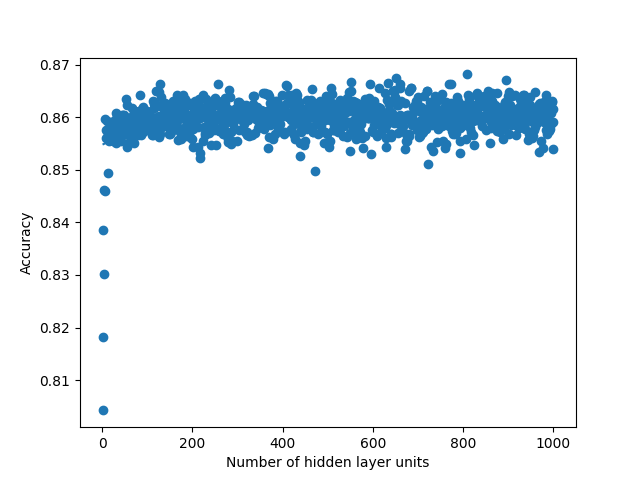
\includegraphics[width=0.8\linewidth]{figures/1000_iterations_churn.png}
    \setlength{\belowcaptionskip}{-15pt}
    \caption{Accuracy vs Number of hidden layers}
    \label{dnadigest}
\end{figure}

\subsection{Titanic Model}

\begin{figure}[H]
    \centering
    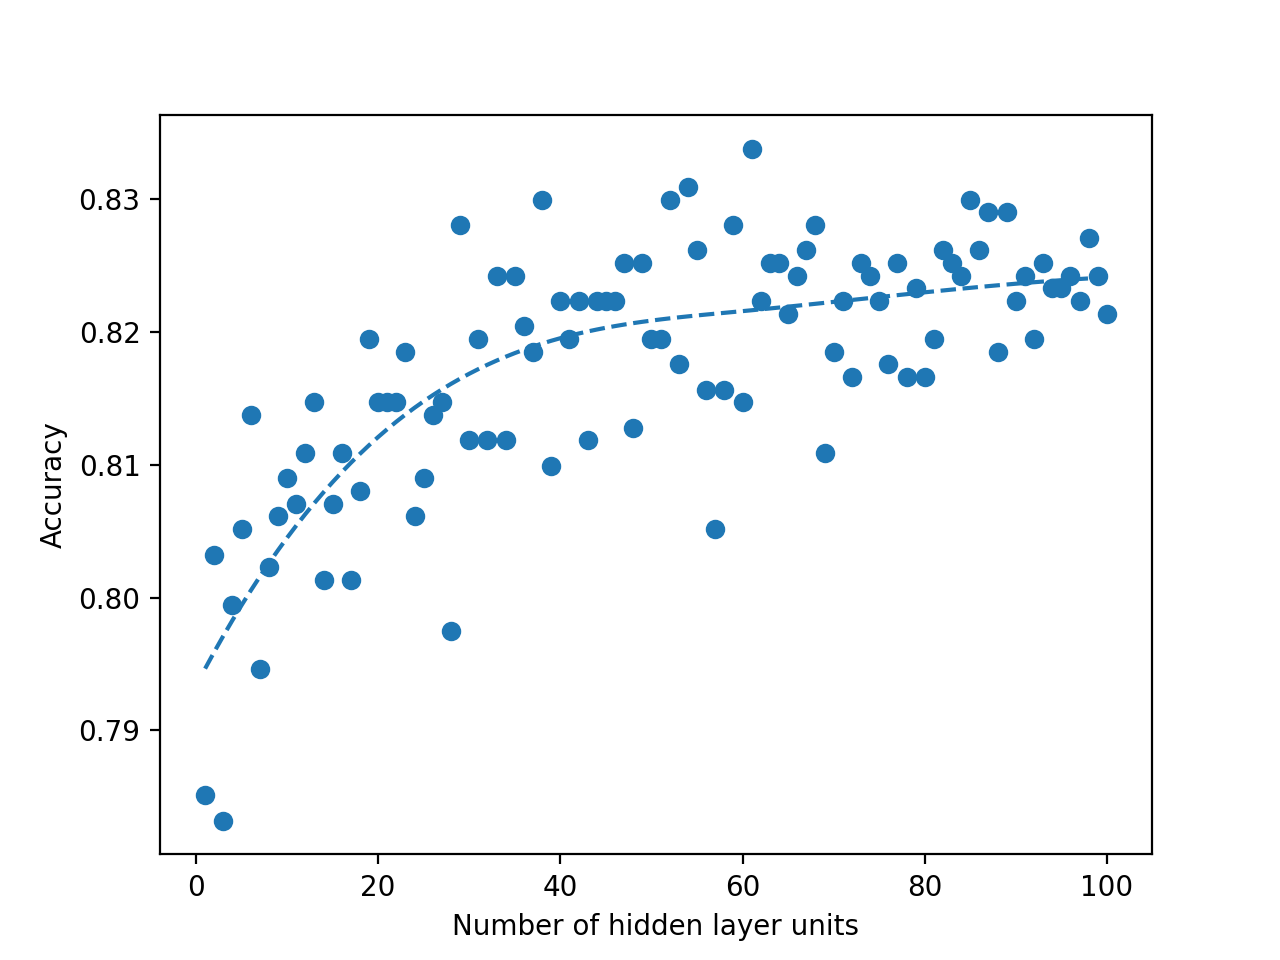
\includegraphics[width=0.8\linewidth]{figures/drexelai_binary_search_train_acc_titanic.png}
    \setlength{\belowcaptionskip}{-15pt}
    \caption{Accuracy vs Number of hidden layers}
    \label{dnadigest}
\end{figure}


\begin{figure}[H]
    \centering
    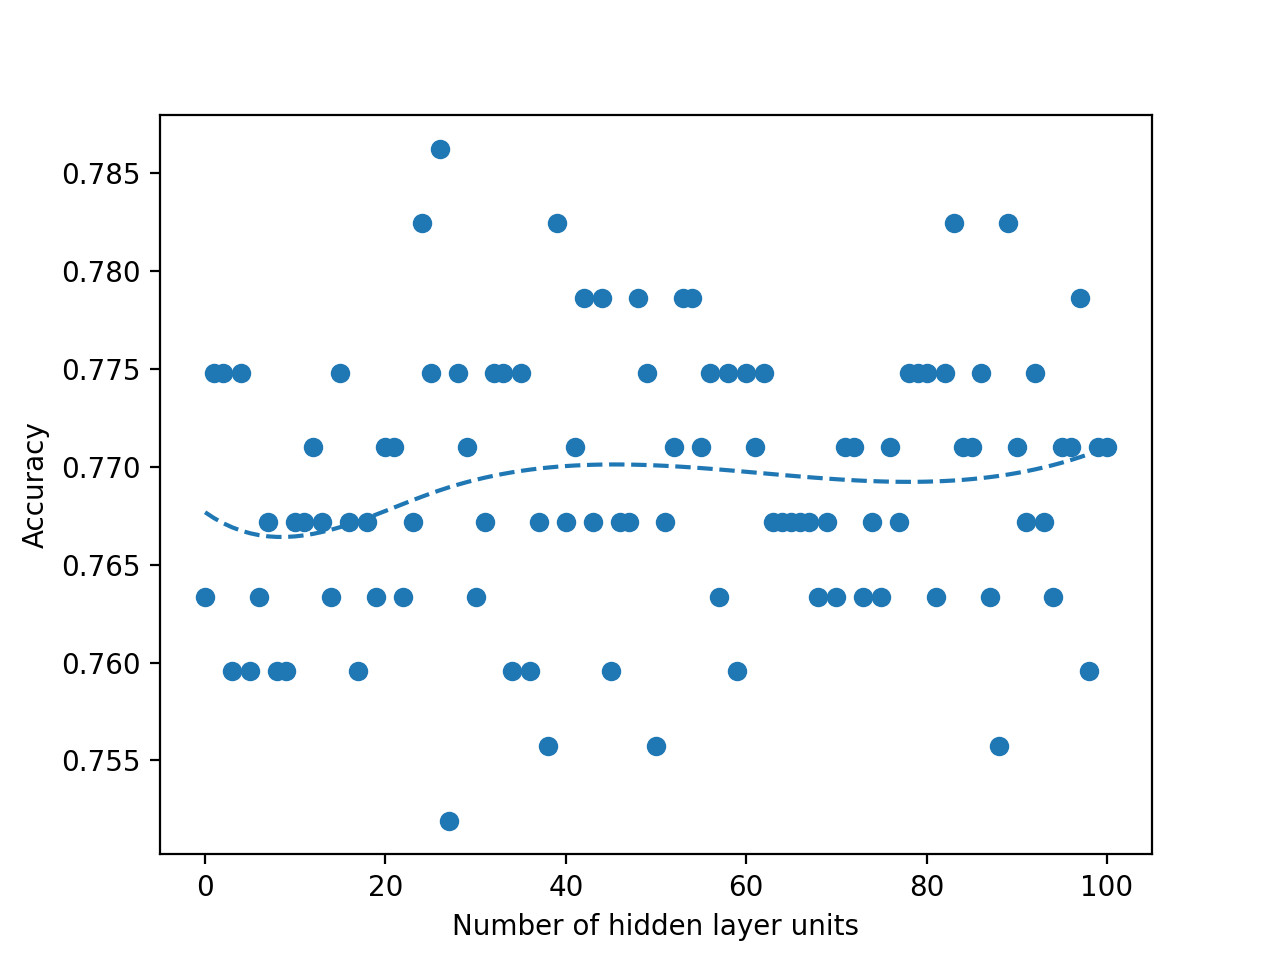
\includegraphics[width=0.8\linewidth]{figures/drexelai_binary_search_test_acc_titanic.png}
    \setlength{\belowcaptionskip}{-15pt}
    \caption{Accuracy vs Number of hidden layers}
    \label{dnadigest}
\end{figure}


% TODO
\begin{figure}[H]
    \centering
    \includegraphics[width=0.8\linewidth]{figures/placeholder.png}
    \setlength{\belowcaptionskip}{-15pt}
    \caption{When applied linear search}
    \label{dnadigest}
\end{figure}

% TODO
\begin{figure}[H]
    \centering
    \includegraphics[width=0.8\linewidth]{figures/placeholder.png}
    \setlength{\belowcaptionskip}{-15pt}
    \caption{When applied binary search}
    \label{dnadigest}
\end{figure}



\section{Conclusion}\label{conclusion}

In this paper, we propose a framework to find the optimal architecture size for any binary classification problem. We employ linear search and binary search to find such architecture size to give the highest accuracy. We use the Titanic dataset and the Churn Rate dataset for our research find out how to apply binary search on any binary classification problem with our assumptions that we explain in the paper. 

\section{Future Work}
We hope to remove some of the relaxations by augmenting the data to fit a cusp. In this paper, we assumed that the accuracy when plotted against the neuron number in the hidden layer would then go up and then come down. We assumed that the accuracy graph when plotted against the architecture size would not be strictly monotonically increasing. In the future, we can look into removing this assumption in order to generalize the approach to all datasets


\section*{Acknowledgment}

We would like to acknowledge Drexel Society of Artificial Intelligence for its contributions and support for this research. 


\begin{thebibliography}{00}

\bibitem{titanickaggledataset} Titanic Kaggle Dataset, \url{https://www.kaggle.com/c/titanic-dataset/data}

\bibitem{churndataset}Churn Customer Prediction Dataset, published by Drexel Society of Artificial Intelligence, December, 2021, \url{https://github.com/drexelai/binary-search-in-neural-nets/blob/main/ChurnModel.csv}

\end{thebibliography}

\end{document}
